\documentclass{beamer}

%%%%% ===== 设置主题 *****
\usetheme{Berlin}
% 可供选择的主题参见 beameruserguide.pdf
% 无导航条的主题: Bergen, Boadilla, Madrid, CambridgeUS,
%                 GoettingenAnnArbor,Pittsburgh, Rochester;
% 有树形导航条的主题: Antibes, JuanLesPins, Montpellier;
% 有目录竖条的主题: Berkeley, PaloAlto, Goettingen, Marburg, Hannover;
% 有圆点导航条的主题: Berlin, Ilmenau, Dresden, Darmstadt, Frankfurt, Singapore, Szeged;
% 有节与小节导航条的主题: Copenhagen, Luebeck, Warsaw

\useinnertheme{circles}
\useoutertheme{infolines}
\usefonttheme[onlymath]{serif}
\setbeamertemplate{navigation symbols}{} % remove the navigation
\setbeamersize{text margin left=0.8cm, text margin right=0.8cm}
\setbeamerfont{frametitle}{size=\large}
\setbeamerfont{footline}{family=\ttfamily}\setbeamertemplate{caption}[numbered]
%%%%% ===== 宏包 *****
\usepackage{amsmath,amssymb,amsfonts}
\usepackage{graphicx,xcolor}
\usepackage{hyperref}
\usepackage{bm}
\usepackage{amsthm}
\usepackage{ulem}
% \usepackage{algorithmicx,algorithm}
\usepackage[linesnumbered,ruled,vlined]{algorithm2e}
\usepackage{fontspec}
\usepackage{xeCJK}
%\usepackage{biblatex}
%\bibliographystyle{plain}
\usepackage[backend=bibtex,style=numeric,sorting=none]{biblatex}
%\addbibresource{example.bib} %BibTeX数据文件及位置
\addbibresource{bibtex3.bib}
\setbeamerfont{footnote}{size=\tiny}
%\usepackage[round,sort&compress]{natbib}
\renewcommand{\baselinestretch}{1.1}

%%%%% ===== 自定义命令 *****
\newcommand{\myem}[1]{\textcolor{blue}{#1}}
\renewcommand{\today}{\number\year 年\number\month 月\number\day 日}
\renewcommand{\figurename}{图}
%\newtheorem{theorem}{Theorem}

\begin{document}
\title[新能源与储能容量配置优化研究]%
{新能源与储能容量配置优化研究}


\author[杜洪博]%
{报告人: 杜洪博\\
导\quad 师: 寇彩霞\rule[0pt]{0pt}{20pt}\\}

\institute[BUPT]{\textcolor[rgb]{0.0,0.0,0.10}%
{\small\ttfamily 北京邮电大学\ 理学院\\[10pt]}}

\date{\today}

% ===== title page ====================================
\begin{frame}[plain]
	\titlepage
\end{frame}

\begin{frame}
	\frametitle{目录}
	\tableofcontents[hideallsubsections] %[pausesections]
\end{frame}

\AtBeginSection[] % Do nothing for \section*
{ \begin{frame}<beamer> %\frametitle{Outline}
		\tableofcontents[currentsection,hideallsubsections]%,currentsubsection]
	\end{frame}
}

%===== Main part start here ==========================
%===== 开题报告 =======================================

\section{问题背景与研究意义}

\begin{frame}
	\frametitle{问题背景} 
	\qquad 我国沙漠、戈壁、荒漠地区风能、太阳能资源丰富,习近平总书记在《生物多样性公约》第十五次缔约方大会领导人峰会主旨讲话中提出,中国将大力发展新能源,在沙漠、戈壁、荒漠地区加快规划建设大型风电光伏基地项目[1]。建设“沙戈荒”大型新能源基地是实现我国“碳达峰、碳中和”目标的重要举措[2]。
\end{frame}

\begin{frame}
	\frametitle{研究意义} 
	\qquad 预计到2030年,国家规划建设了约4.55亿千瓦的“沙戈荒”新能源基地,“沙戈荒”新能源基地以风光火储多能互补一体化形式,通过特高压直流通道将清洁电力外送至中东部负荷中心消纳,是我国未来新能源消纳的重要形式[3]。

	\qquad 所以为了提高系统的经济性、可靠性,在规划阶段如何合理配置新能源电源及储能的容量是一个重要的研究问题。

\end{frame}

\section{研究现状}

\begin{frame}
	\frametitle{研究现状} 
    文献[9]研究了支撑新能源基地电力外送的电源组合优化配置策略,测算了新能源基地为满足通道利用率和运行经济性所需配置的电化学储能装机占比。
	
	文献[10]针对系统友好型“无火电”能源大基地构建开展研究,从经济性、调峰、一次调频、惯例响应等方面评估了新能源与储能在能源大基地中对火电机组的替代作用。
	
	文献[11]提出了电力系统源-网-储灵活性资源协调优化规划模型,考虑各类灵活性资源约束,从不同时间和空间尺度统筹优化新能源电源、储能及电网互联容量。
\end{frame}

\begin{frame}
	\frametitle{研究现状} 
	文献[12]提出了一种基于多目标规划的光伏电站+光热电站的混合优化配置方法。
	
	文献[13]针对含风电、光伏、光热、火电、水电的多能互补系统,提出了一种两阶段优化的光热电站镜场、发电装机和储热容量的协调优化配置方法。

	已有研究主要面向电源侧多能互补发电系统,针对“沙戈荒”大规模基地的新能源与储能协调优化配置的研究还较为少见。
\end{frame}

\section{研究内容与方法}

\begin{frame}
	\frametitle{系统结构} 
	图\ref*{fig.1}给出了简化后系统的整体结构示意。系统内新能源基地采用风光火储多能互补一体化的形式,通过特高压直流外送通道将清洁电力向受端电网输送。
	\begin{figure}[htbp]  
		\centering  
		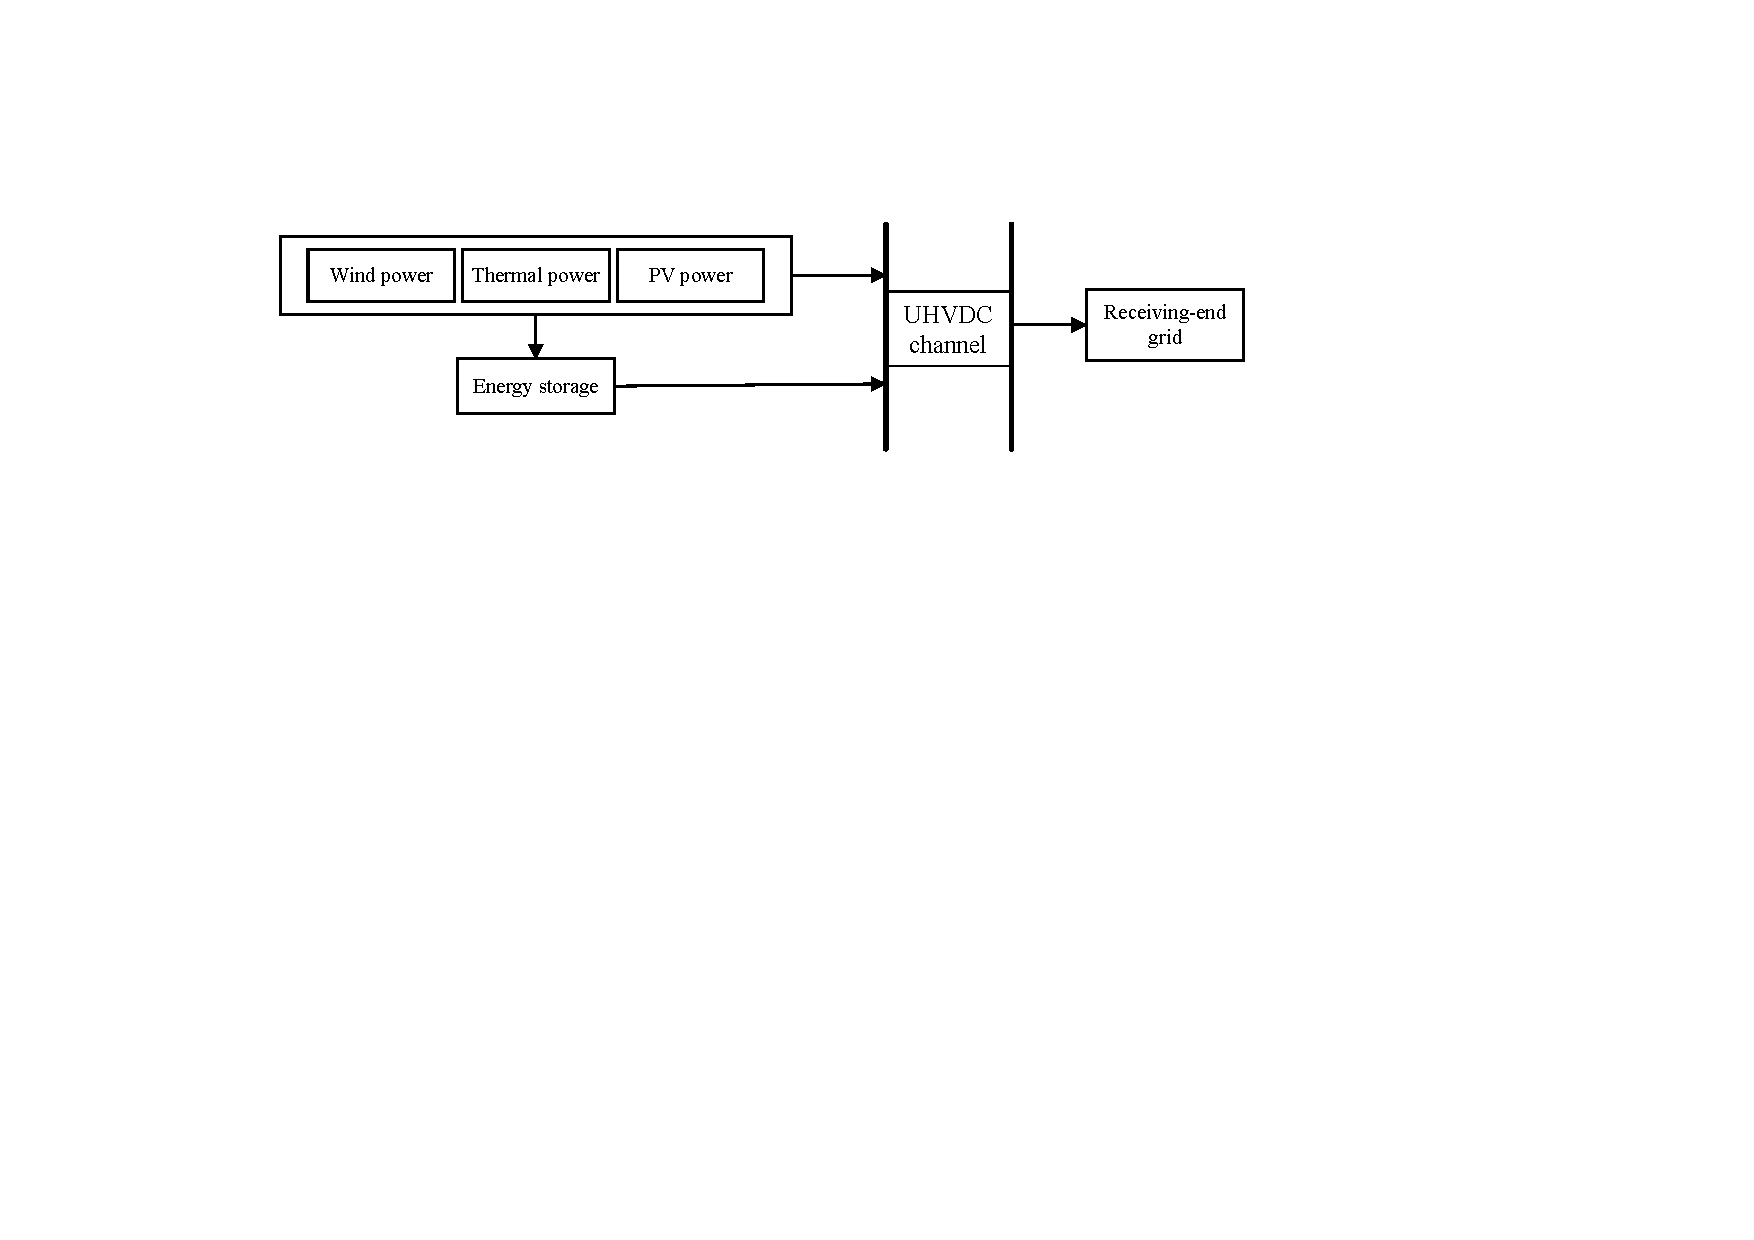
\includegraphics[scale=0.6]{./pic/系统结构示意图.pdf}
		\caption{系统结构示意图}
		\label{fig.1}
	\end{figure}
	在此系统上以总投资成本最小为目标,考虑新能源发电量占比、新能源利用率、储能电站运行、火电机组运行与外送通道等约束,建立风光储系统容量优化模型。
\end{frame}

\begin{frame}
	\frametitle{研究内容} 
	
\end{frame}

\begin{frame}
	\frametitle{研究方法} 

\end{frame}

\section{未来工作安排}
\begin{frame}
	\frametitle{未来工作安排} 
	1.阅读文献,并查找相关数据,丰富数值实验;

	2.继续探索提高求解效率和求解质量的方法;

	3.完善模型,使容量配置优化模型更符合实际情况。
\end{frame}



% ====== End =========================================
\begin{frame}
\vspace{1em}
\centering
\textcolor{black}{\LARGE\bf 谢谢各位老师和同学!}

\end{frame}

\end{document}
